


%Due to the rapid expansion of scientific literature, it is challenging for researchers to stay up-to-date on the latest developments even within a narrow subfield.
%It is challenging for researchers to stay up-to-date and verify scientific findings due to the rapid expansion of scientific literature. developments in scientific literature due to the rapid changing and uncertain information that occurs frequently  even within a narrow subfield

Due to rapid growth in the scientific literature, it is difficult for researchers -- and the general public even more so -- to stay up to date on the latest findings. This challenge is especially acute during public health crises like the current COVID-19 pandemic, due to the extremely fast rate at which new findings are reported and the risks associated with making decisions based on outdated or incomplete information. %Therefore, it is very challenging for researchers and public to stay up-to-date  with the latest developments.
As a result, there is a need for automated tools to assist researchers and the public in evaluating the veracity of scientific claims. % in light of the latest evidence. %This need is especially urgent when high-stakes decisions must be made based on rapidly changing and uncertain information, a situation that occurs frequently during public health crises like the current COVID-19 pandemic.


\emph{Fact-checking} -- a task in which the veracity of an input \emph{claim} is verified against a corpus of documents that \emph{support} or \emph{refute} the claim -- has been studied to combat the proliferation of misinformation in political news, social media, and on the web~\cite{Thorne2018FEVERAL,Hanselowski2019ARA}. However, verifying scientific claims poses new challenges to both dataset construction and effective modeling. While political claims are readily available on fact-checking websites and can be verified by crowd workers, annotators with extensive domain knowledge are required to generate and verify scientific claims. In addition, NLP systems for scientific claim verification must possess expert background knowledge, as well as language understanding and reasoning capabilities not required to verify factoid claims. % In turn, interest in fact-checking has spurred the creation of many datasets across different domains to support research and development of automated fact-checking systems \hanna{add citations}.

\begin{figure}[t]
  \centering

  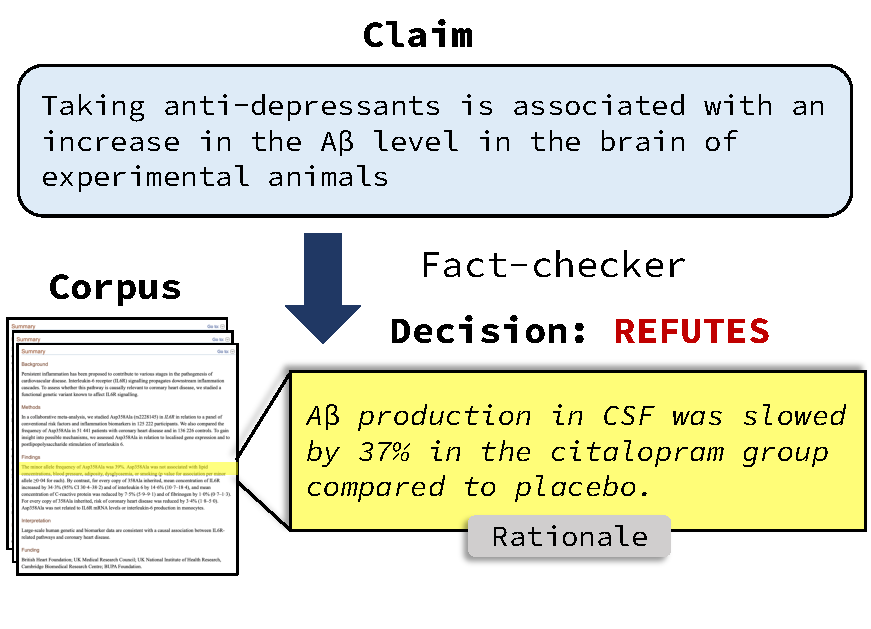
\includegraphics[width=\columnwidth]{figures/teaser-fig.pdf}
  \caption{A \ours claim refuted by evidence. To refute this claim, the system must recognize that (1) ``CSF'' is an acronym for ``cerebral spinal fluid'', found in the brain, (2) ``Citalopram'' is a type of antidepressant, but ``placebo'' is not, and (3) ``Slowing by 37\%'' indicates a reversal in effect relative to the claim.}
  \label{fig:teaser}
\end{figure}
\definecolor{c1}{RGB}{84,130,53}
% \newcommand{\supportsCovid}[1]{{\color{c1} \textbf{#1}}}
\newcommand{\supportsCovid}[1]{{\color{c1} {#1}}}

\definecolor{c2}{RGB}{218,0,0}
% \newcommand{\refutesCovid}[1]{{\color{c2} \textbf{#1}}}
\newcommand{\refutesCovid}[1]{{\color{c2} {#1}}}

\definecolor{c3}{RGB}{127,127,127}
\newcommand{\wrongContext}[1]{{\color{c3} \textbf{#1}}}



\begin{table*}[t!]
  \setlength{\tabcolsep}{.25em}
  \footnotesize
  \centering

  \begin{tabularx}{\textwidth}{ X }
    \toprule
    \textbf{Claim 1}: Lopinavir / ritonavir have exhibited favorable clinical responses when used as a treatment for coronavirus. \\
    \midrule
    \textbf{Supports}: \dots \supportsCovid{Interestingly, after lopinavir/ritonavir (Kaletra, AbbVie) was administered, $\beta$-coronavirus viral loads significantly decreased and no or little coronavirus titers were observed.} \\
    \midrule
    \textbf{Refutes}: \refutesCovid{The focused drug repurposing of known approved drugs (such as lopinavir/ritonavir) has been reported failed for curing SARS-CoV-2 infected patients.}. It is urgent to generate new chemical entities against this virus \dots \\
    \midrule
    \textbf{Claim 2}: The coronavirus cannot thrive in warmer climates. \\
    \midrule
    \textbf{Supports}: \supportsCovid{...most outbreaks display a pattern of clustering in relatively cool and dry areas...This is because the environment can mediate human-to-human transmission of SARS-CoV-2, and unsuitable climates can cause the virus to destabilize quickly...} \\
    \midrule
    \textbf{Refutes}: \refutesCovid{...significant cases in the coming months are likely to occur in more humid (warmer) climates, irrespective of the climate-dependence of transmission and that summer temperatures will not substrantially limit pandemic growth}. \\
    \bottomrule
  \end{tabularx}

  \caption{Evidence identified by our system as supporting and refuting two claims concerning COVID-19.}
  \label{tbl:covid_example}


\end{table*}

In this paper, we introduce the task of scientific claim verification (Figure~\ref{fig:teaser}) to evaluate the veracity of scientific claims against a research corpus. Table \ref{tbl:covid_example} presents some examples. To facilitate research on this task, we construct \ours, an expert-annotated dataset of \numclaims scientific claims accompanied by scientific abstracts that support or refute each claim, and annotated with rationales \cite{Lei2016RationalizingNP} justifying each support / refute decision. To create the dataset, we develop a novel annotation protocol in which annotators re-formulate naturally occurring claims in the scientific literature -- \emph{citation sentences} -- into atomic scientific claims. Using citation sentences as a source of claims both speeds the claim generation process and guarantees that the topics discussed in \ours are representative of the research literature. In addition, citation links indicate the exact documents likely to contain evidence necessary to verify a given claim.

We establish performance baselines on \ours following \citet{DeYoung2019ERASERAB}, which achieves strong performance on \fever, a Wikipedia fact checking dataset~\cite{Thorne2018FEVERAL}. Our baseline is a pipeline system which retrieves abstracts related to an input claim, uses a \bert-based \cite{Devlin2019BERTPO} sentence selector to identify rationale sentences, and labels each abstract as \supports, \refutes, or \notenough with respect to the claim. We show that our baseline can benefit from training on fact-checking data from domains including Wikipedia articles and politics.  %46.5 F1 in verifying claims and identifying rationales. data adapts fact-checking models trained on Wikipedia articles and political news and fine-tuned on

%pipeline model following the ``\bert-to-\bert'' approach from \citet{DeYoung2019ERASERAB}, which achieves strong performance on \fever.  Our model, which we call \sysname, \dw{From Sewon: What are new components compared to DeYoung? If they are mostly same as DeYoung, not sure if giving it a new name is a great idea} retrieves abstracts related to a given claim, uses a \bert-based \cite{Devlin2019BERTPO} sentence selector to identify rationale sentences, and then labels each claim as \supports, \refutes, or \notenough with respect to the claim. Our system is able to identify correctly-labeled and rationalized evidence abstracts with performance of 46.5 F1, indicating that the task is doable but leaving ample room for improvement \dw{From Bhargavi: what's an upper bound from domain experts? How can we contextualize 46 somehow?}. Despite its small size, training \sysname on \ours leads to better performance than training on fact-checking datasets constructed from Wikipedia articles \cite{Thorne2018FEVERAL} and political news \cite{Hanselowski2019ARA}. The strongest performance is achieved using a simple domain adaptation strategy, pretraining on \fever and then finetuning on \ours.

We showcase the ability of our model to verify expert-written claims concerning the novel coronavirus COVID-19 against the newly-released CORD-19 corpus \cite{Wang2020CORD19TC}. Expert annotators judge retrieved evidence to be plausible for 23 of 36 claims.\footnote{We emphasize that our model is a \emph{research prototype} and should not be used to make any medical decisions whatsoever.} Our results and analyses demonstrate the importance of the new task and dataset to support significant future research in this domain.
% Uncomment for camera-ready.
% Our data and models will be released publicly at \website.